\documentclass[floatfix,nofootinbib,superscriptaddress,fleqn]{revtex4-2} 
%\documentclass[aps,epsfig,tightlines,fleqn]{revtex4}
\usepackage[utf]{kotex}
\usepackage[HWP]{dhucs-interword}
\usepackage[dvips]{color}
\usepackage{graphicx}
\usepackage{bm}
%\usepackage{fancyhdr}
%\usepackage{dcolumn}
\usepackage{defcolor}
\usepackage{amsmath}
\usepackage{amsfonts}
\usepackage{amssymb}
\usepackage{amscd}
\usepackage{amsthm}
\usepackage[utf8]{inputenc}
 \usepackage{setspace}
 \usepackage{tikz}
%\pagestyle{fancy}

\begin{document}

\title{\Large 2022년 1학기 물리학 I: Quiz 10}
\author{김현철\footnote{Office: 5S-436D (면담시간 매주
    화요일-16:00$\sim$20:00)}} 
\email{hchkim@inha.ac.kr}
\author{Lee Hui-Jae} 
\email{hjlee6674@inha.edu}
\affiliation{Hadron Theory Group, Department of Physics,
Inha University, Incheon 22212, Republic of Korea }
\date{Spring semester, 2022}

\maketitle

\noindent {\bf 문제 1. (30pt)} 
그림~\ref{fig:2}에서처럼
$\theta=30.0^\circ$만큼 기울어져 있는 면 위에 질량이 12.0 kg인
나무토막이 놓여있다. 이 토막 아래에는 270. N의 힘을 받으면 2.00 cm만큼 
압축되는 용수철이 놓여있다. 이 토박을 가만히 놓으면, 비탈면으로
내려와서 용수철을 5.50 cm 압축시킨다.
\begin{figure}[ht]
  \centering
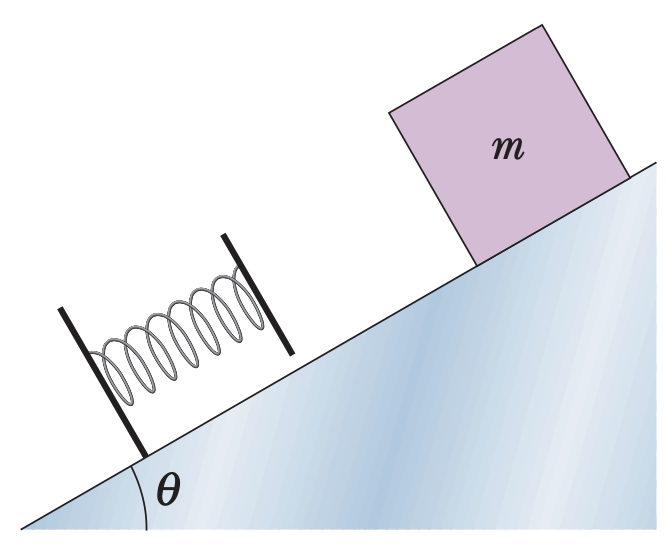
\includegraphics[scale=0.5]{Qfig9-2-20210330.png}  
  \caption{문제 1}
  \label{fig:2}
\end{figure}

\begin{itemize}
\item[(가)] 정지 상태에서 용수철을 압축시켜 멈추게 될 때까지 이
  나무토막은 얼마나 내려왔는가?
\item[(나)] 나무토막이 용수철에 닿는 순간의 속력은 얼마인가?   
\end{itemize}

\noindent {\bf 풀이 : } 
\begin{itemize}
  \item[(가)]
  나무 토막 비탈면을 내려올 때와 
  용수철을 압축시켜 정지해 있을 때의 자유 물체 다이어그램을 그려보자. 
  \begin{figure}[htbp]
    \centering
    \begin{tikzpicture}
      \draw node[] at (-2,2) {하강 : };
      \draw[rotate=30] (0,-2) -- (0,1.5); 
      \draw[rotate=30] (-2.5,0) -- (2.5,0);
  
      \draw[red,very thick,-latex] (0,-0.1) -- (0,-2) 
      node [left,black] {$F_g$};
      \draw[rotate=30,blue,very thick,-latex] (0,0.1)--(0,1.28)
      node [above,black,right] {$N$};
      \draw[] (0,-0.5) arc(270:300:0.5) (0,0.5)
      node [below=45,right=-2.5] {$30^\circ$};
    \end{tikzpicture}
    \hspace{1.5cm}
    \begin{tikzpicture}
      \draw node[] at (-2,2) {정지 : };
      \draw[rotate=30] (0,-2) -- (0,1.5); 
      \draw[rotate=30] (-2.5,0) -- (2.5,0);
  
      \draw[red,very thick,-latex] (0,-0.1) -- (0,-2) 
      node [left,black] {$F_g$};
      \draw[rotate=30,blue,very thick,-latex] (0,0.1)--(0,1.28)
      node [above,black,right] {$N$};
      \draw[violet,rotate=30,very thick,-latex] (0.1,0)--(1,0)
      node [above,black] {$f_s$};
      \draw[] (0,-0.5) arc(270:300:0.5) (0,0.5)
      node [below=45,right=-2.5] {$30^\circ$};
    \end{tikzpicture}\caption{자유 물체 다이어그램}
  \end{figure}
  나무토막은 처음에 정지해 있었으므로 초기에 가지고 있던 역학적 에너지를 $E_i$, 
  나무토막이 비탈면을 내려온 거리를 $d$라 하자. 즉 $d$는 나무토막이 정지해 있던 
  지점에서 용수철에 의해 정지한 지점까지의 직선 거리이다. 그러면,
  \begin{align}
    E_i = mgh = mgd\sin{\theta},\,\,\, m = 12.0\,\mathrm{kg}.
  \end{align}
  나무토막이 용수철을 압축시켜 정지하였으므로 나무토막이 가지고 있던 모든 역학적 에너지가
  용수철의 탄성 위치에너지로 전환되었다. 용수철이 압축된 길이를 $x_f$라고 하면,
  \begin{align}\label{eq:1-1}
    E_i = mgd\sin{\theta} = \frac{1}{2}kx_f^2,\,\,\, x_f = 5.50\,\mathrm{cm}
    =5.50\times 10^{-2}\mathrm{m}.
  \end{align}
  용수철은 270 N의 힘을 받을 때 2.00 cm만큼 압축되므로 용수철 상수 $k$는,
  \begin{align}
    k = \frac{F}{x} = \frac{270\,\mathrm{N}}{2.00\,\mathrm{cm}}
    = \frac{270\,\mathrm{N}}{2.00\times 10^{-2}\,\mathrm{m}}.
  \end{align}
  식 (\ref{eq:1-1})에 의해 나무토막이 내려온 거리 $d$는 다음과 같다.
  \begin{align}
    \begin{split}
      d &= \frac{kx_f^2}{2mg\sin{\theta}}
      =\frac{(270\,\mathrm{N})(5.50\times 10^{-2}\mathrm{m})^2}
      {2(2.00\times 10^{-2}\,\mathrm{m})(12.0\,\mathrm{kg})
      (9.80\,\mathrm{m/s^2})\sin{30.0^\circ}} \\
      &= 3.47\times 10^{-1}\mathrm{m}  \\
      &=34.7\,\mathrm{cm}.
    \end{split}
  \end{align}
  \item[(나)] 용수철에 닿는 순간의 역학적 에너지를 $E_s$, 이 때와 나무토막이 
  정지한 지점 사이의 직선 거리를 $d_s$라고 하면,
  \begin{align}
    E_s = \frac{1}{2}mv^2+mgd_s\sin{\theta},\,\,\,d_s = 5.50\,\mathrm{cm}
    =5.50\times 10^{-2}\mathrm{m}.
  \end{align}
  역학적 에너지는 보존되어야 하므로 이 에너지는 처음 역학적 에너지 $E_i$와 같다. 따라서,
  \begin{align}
    E_s = E_i,\,\,\,\frac{1}{2}mv^2+mgd_s\sin{\theta} = mgd\sin{\theta}.
  \end{align}
  따라서 이 때의 속력은,
  \begin{align}
    \begin{split}
      v &= \sqrt{2gd\sin{\theta}-2gd_s\sin{\theta}}
      = \sqrt{2g(d-d_s)\sin{\theta}}  \\
      &= \sqrt{2(9.80\,\mathrm{m/s^2})
      \left((3.47\times 10^{-1}\mathrm{m})
      -(5.50\times 10^{-2}\mathrm{m})\right)
      \sin{30.0^\circ}} \\
      &= 1.69\,\mathrm{m/s}.
    \end{split}
  \end{align}
\end{itemize}

\vspace{1cm}

\noindent {\bf 문제 2. (50 pt)(\textcolor{red}{난이도 상})}
어떤 아이가 그림~\ref{fig:2}처럼
반지름이 $R$인 반구 모양의 얼음 위에 앉아 있다가 무시할 수 있는 아주
작은 처음속력으로 미끄러지기 시작한다. 

\begin{figure}[ht]
  \centering
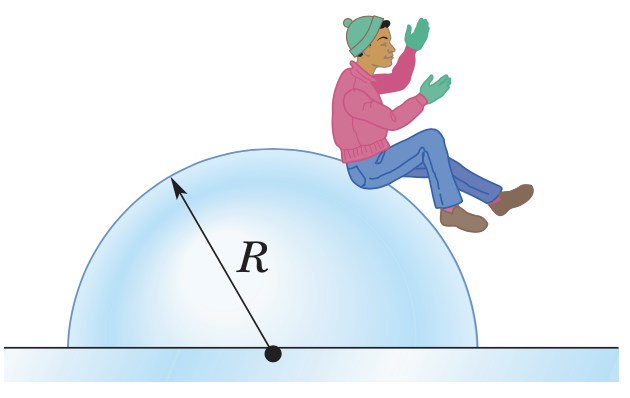
\includegraphics[scale=0.5]{Qfig9-3-20210330.png}  
  \caption{문제 2}
  \label{fig:2}
\end{figure}

얼음과 아이 사이에 쓸림이 없다고 가정한다면, 아이가 얼음에서 떠나는
높이는 어디인가?

\noindent {\bf 풀이 : } 
아이의 얼음을 떠나는 순간의 자유 물체 다이어그램은 다음과 같다.
\begin{figure}[htbp] 
  \centering
  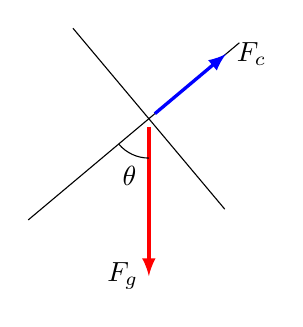
\begin{tikzpicture}
    \draw[rotate=-50] (0,-2) -- (0,1.5); 
    \draw[rotate=-50] (-1.5,0) -- (1.5,0);

    \draw[red,very thick,-latex] (0,-0.1) -- (0,-2) 
    node [left,black] {$F_g$};
    \draw[rotate=-50,blue,very thick,-latex] (0,0.1)--(0,1.28)
    node [above,black,right] {$F_c$};
    \draw[] (0,-0.5) arc(270:220:0.5) (0,0.5)
    node [below=35,left=1] {$\theta$};
  \end{tikzpicture}\caption{얼음을 떠날 때의 다이어그램}
\end{figure}
아이는 얼음 위에서 원궤도를 그리며 떨어지므로 원심력 $F_c$가 존재한다. 
중심 방향으로 작용하는 중력의 크기가 원심력보다 작아질 때 아이는 얼음을 떠난다.
즉,
\begin{align}\label{eq:2-1}
  F_g\cos{\theta} \leq F_c,\,\,\,F_g = mg
\end{align}
일 때 아이는 얼음을 떠난다. 역학적 에너지 보존 법칙을 이용하기 위해 
아이의 처음 역학적 에너지를 $E_i$라 하자. 
아이는 처음에 정지해 있었으므로,
\begin{align}
  E_i = mgR.
\end{align}
얼음에서 떠나는 순간의 역학적 에너지를 $E_f$, 그 때의 높이와 속력을 
$R_f$, $v_f$라 하면 아이가 얼음을 떠나는 순간 지면에서의 높이 
$R_f$를 얼음의 반지름 $R$과 $\theta$의 삼각비로 표현할 수 있다.
\begin{align}
  E_f = mgR_f + \frac{1}{2}mv_f^2,\,\,\,R_f=R\cos{\theta}.
\end{align}
 역학적 에너지는 보존되므로,
\begin{align}
  mgR = mgR_f + \frac{1}{2}mv_f^2.
\end{align}
이 때 작용하는 원심력 $F_c$는,
\begin{align}
  F_c = \frac{mv_f^2}{R} = \frac{2mg(R-R_f)}{R}
  = 2mg\left(1-\cos{\theta}\right),
\end{align}
이므로 식 (\ref{eq:2-1})에 의해,
\begin{align}
  mg\cos{\theta} \leq 2mg\left(1-\cos{\theta}\right),\,\,\,
  \cos{\theta} \leq \frac{2}{3}.
\end{align}
따라서,
\begin{align}
  R_f = R\cos{\theta} \leq \frac{2}{3}R,
\end{align}
아이의 높이가 $\frac{2}{3}R$인 순간 부터 얼음을 벗어난다.

\vspace{1cm}

\noindent {\bf 문제 3. (20 pt)}
그림~\ref{fig:3}의 암모니아 분자($\mathrm{NH}_3$)는 세 개의
수소원자(H)가 정삼각형의 꼭지점에 있고 정삼각형의 중심은
수소원자로부터 $d=9.40\times 10^{-11}$ m만큼 떨어져
있다. 질소원자(N)는 수소원자들이 바닥을 이루는 피라미드의 꼭지점에
있다. 질소 대 수소의 원자질량 비율은 13.9이고, 질소에서 수소까지의
거리는 $L=10.14\times 10^{-11}$ m이다. 

\begin{figure}[ht]
  \centering
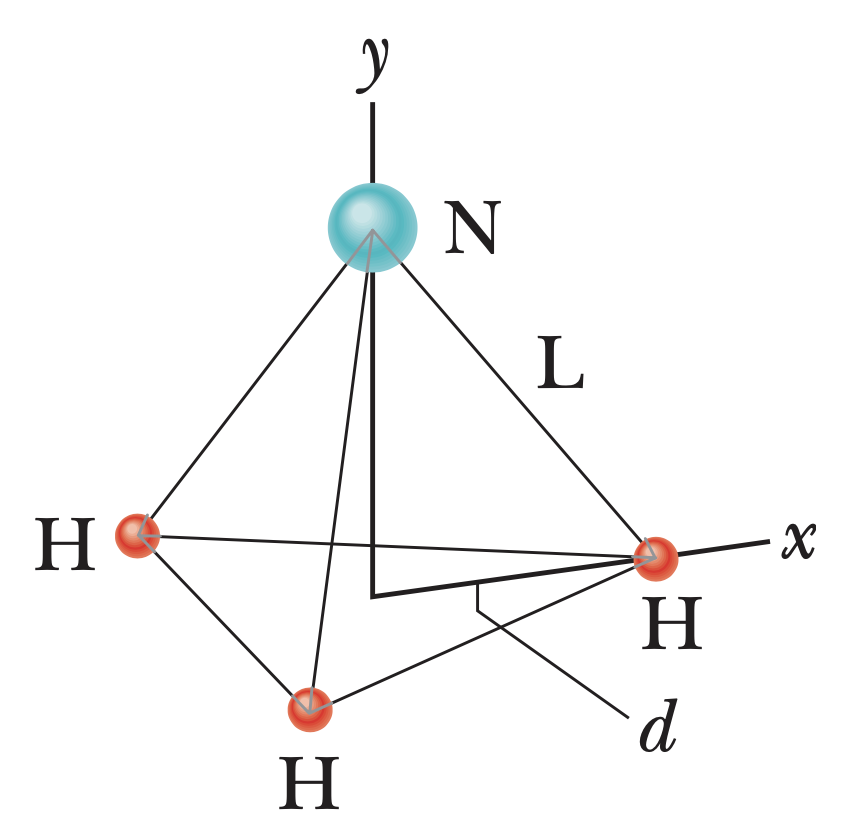
\includegraphics[scale=0.3]{Qfig9-4-20220330.png}  
  \caption{문제 3}
  \label{fig:3}
\end{figure}

암모니아분자의 질량중심의
\begin{itemize}
\item[(가)] $x$ 좌표
\item[(나)] $y$ 좌표는 각각 무엇인가? 
\end{itemize}

\noindent {\bf 풀이 : } 

\begin{itemize}
  \item[(가)] 

  \begin{figure}[htbp]
    \centering
    \begin{tikzpicture}
      \draw (0:-2.5) -- (0:2.5)
      node[above] {$x$};
      \coordinate (A) at (0:1.5)
      node[above] at (A) {$H1$};
      \coordinate (B) at (120:1.5)
      node[above] at (B) {$H2$};
      \coordinate (C) at (240:1.5)
      node[below] at (C) {$H3$};
      \draw (A) -- (B);
      \draw (B) -- (C);
      \draw (C) -- (A);
      \coordinate (O) at (0,0);
      \draw node[above] at (O) {$N$};
      \draw[dotted] (O) -- (B);
      \draw[dotted] (O) -- (C);
      \draw[dotted] (O) -- (A);
    \end{tikzpicture}\caption{위에서 내려다 본 원자들의 위치}
  \end{figure}
  
  정삼각형의 중심을 원점, 
  $x$축 위에 위치한 수소 원자 부터 반시계 방향으로 1, 2, 3번 수소라 
  하자. 질량 중심의 $x$ 좌표를 $x_{cm}$이라 하면 $x_{cm}$은,
  \begin{align}
    x_{cm} = \frac{m_{N}x_{N} + m_{H}x_{H1} + m_{H}x_{H2} + m_{H}x_{H3}}
    {m_{N} + m_{H} + m_{H} + m_{H}}.
  \end{align}
  질소 원자의 $x$ 좌표는 0 이고 각 수소들은 정삼각형의 꼭짓점에 위치하므로,
  \begin{align}
    \begin{split}
      x_{H1} &= d  \\
      x_{H2} &= d\cos{120^\circ} =-\frac{1}{2}d \\
      x_{H3} &= d\cos{240^\circ} =-\frac{1}{2}d .
    \end{split}
  \end{align}
  $x_{cm}$의 분모는 다음과 같이 얻어진다.
  \begin{align}
    \begin{split}
      m_{N}x_{N} + m_{H}x_{H1} + m_{H}x_{H2} + m_{H}x_{H3}
      &=m_{H}\left(d -\frac{1}{2}d -\frac{1}{2}d\right) \\
      &=0
    \end{split}
  \end{align}
  따라서 $x_{cm}$은 0 이다.
  \item[(나)] 질량 중심의 $y$ 좌표를 $y_{cm}$이라 하면 $y_{cm}$은,
  \begin{align}
    y_{cm} = \frac{m_{N}y_{N} + m_{H}y_{H1} + m_{H}y_{H2} + m_{H}y_{H3}}
    {m_{N} + m_{H} + m_{H} + m_{H}}.
  \end{align}
  모든 수소 원자들은 $y=0$평면에 위치해 있으므로 $y$ 좌표가 0 이다. 즉,
  \begin{align}
    y_{H1}=y_{H2}=y_{H3}=0.
  \end{align}
  그림~\ref{fig:3}로 부터 질소 원자의 $y$ 좌표는,
  \begin{align}
    y_{N} = \sqrt{L^2-d^2},
  \end{align}
  이고 질소 대 수소의 원자질량 비율이 13.9 이므로,
  \begin{align}
    \frac{m_N}{m_H} = 13.9,\,\,\,m_{N}=13.9m_{H}.
  \end{align}
  따라서 $y_{cm}$의 분모는 다음과 같다.
  \begin{align}
    m_{N}y_{N} + m_{H}y_{H1} + m_{H}y_{H2} + m_{H}y_{H3}=
    13.9m_{H}\sqrt{L^2-d^2}.
  \end{align}
  $y_{cm}$은,
  \begin{align}
    \begin{split}
      y_{cm} &= \frac{13.9m_{H}\sqrt{L^2-d^2}}{13.9m_{H} + 3m_{H}}
      = \frac{13.9\sqrt{(10.14\times 10^{-11}\,\mathrm{m})^2
      -(9.40\times 10^{-11}\,\mathrm{m})^2}}{13.9 + 3}  \\
      &= 3.13\times10^{-11}\mathrm{m}.
    \end{split}
  \end{align}
  질량중심의 $y$ 좌표는 $3.13\times10^{-11}$ m이다.
\end{itemize}
\end{document}